\documentclass[12pt]{article}
\usepackage{pylatex}
\usepackage{mpllatex}
\usepackage{geometry}
\usepackage{amsmath}
\usepackage{pgf}
\usepackage{caption}
\usepackage{hyperref}
\usepackage{examples}

% portrait
\geometry{papersize={210mm,297mm},hmargin=2cm,tmargin=1.0cm,bmargin=1.5cm}
\parskip=8pt plus 4pt minus 2pt

% landscape
% \geometry{papersize={297mm,210mm},hmargin=2cm,tmargin=1.0cm,bmargin=1.5cm}
% \parskip=6pt plus 3pt minus 2pt

\begin{document}

\section*{A mixed Maple-Python example}

This example demonstrates a cooperative effort where Maple is used to do the analytic computations while Python is used to plot the data.

The example chosen here is to find and plot the solution to the boundary value problem defined by
\begin{align*}
   \frac{d^2y}{dx^2} + 2 \frac{dy}{dx} +10 y = 0\quad\quad\text{with }y(0)=3,\> y'(0)=0
\end{align*}

This example requires two passes, once for Maple and once for Python (and in that order). This example can be run using

\vspace{5pt}

\begin{lstlisting}
   mpllatex.sh -x -i mixed
   pylatex.sh  -x -i mixed
   pdflatex          mixed
\end{lstlisting}

\vspace{5pt}

Note that the last pair of commands could also be combined as {\small\tt pylatex.sh -i mixed}.

\subsection*{The Maple code}

Here Maple is used to first find the general solution of th differential equation. The boundary conitions are then imposed and finally a uniform sampling of the solution is written to a file for later use by Python and Matplotlib.

\begin{maple}
   # a second order ode
   ode := diff(y(x), x, x) + 2*diff(y(x),x) + 10*y(x) = 0:  # mpl (ans.101,ode)

   # find the general solution
   ans := dsolve(ode):                     # mpl (ans.102,ans)

   # set initial conditions
   ics := y(0) = 3, (D(y))(0) = 0:
   tmp := {ics}:                           # mpl (ans.103,tmp)

   # find the particular solution
    f := rhs(dsolve([ics, ode])):          # mpl (ans.104,f)
   df := diff(f,x):                        # mpl (ans.105,df)

    y := x -> f:
   dy := x -> df:

   # now sample y and dy at selected points
   a,b,n := 0.0,2.0*Pi,300:        # domain and number of samples
   dx := (b-a)/n:                  # uniform step

   fd := fopen ("mixed.txt", WRITE):
   for i from 0 to n by 1 do
      x := a + dx*i:
      fprintf(fd,"% .10e % .10e % .10e\n",x,evalf(y(x)),evalf(dy(x))):
   end do:
   fclose(fd):
\end{maple}

The general solution of the differential equation is
\begin{equation*}
  \mpl{ans.102}
\end{equation*}
while the particular solution satifying the boundary conditions is given by
\vspace{5pt}
\begin{align*}
    y(x) &= \mpl{ans.104}
\end{align*}

\subsection*{The Python code}

This is a straighforward use of Matplotlib to plot two functions. The code reads the datafile created previously by Maple and then calls Matplotlib to plot that data.

\begin{python}
   import numpy as np
   import matplotlib.pyplot as plt

   plt.matplotlib.rc('text', usetex = True)
   plt.matplotlib.rc('grid', linestyle = 'dotted')
   plt.matplotlib.rc('figure', figsize = (5.5,4.1)) # (width,height) inches

   x, y, dy = np.loadtxt ('mixed.txt', unpack=True)

   plt.plot (x,y)
   plt.plot (x,dy)

   plt.xlim (0.0,4.0)

   plt.legend(('$y(x)$', '$dy(x)/dx$'), loc = 0)
   plt.xlabel('$x$')
   plt.ylabel('$y(x),\> dy/dx$')
   plt.grid(True)
   plt.tight_layout(0.5)

   plt.savefig('mixed-fig.pdf')
\end{python}

\vspace{10pt}

\begin{minipage}{\textwidth}
   \centering
   \IfFileExists{mixed-fig.pdf}%
   {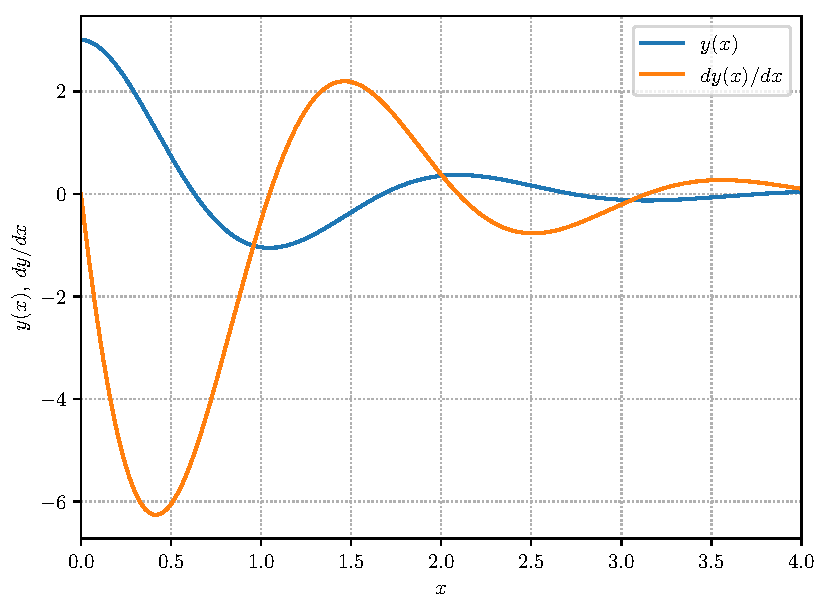
\includegraphics[width=0.75\textwidth]{mixed-fig.pdf}}{Failed to create pdf plot.}
   \captionof{figure}{The function and its derivative.}
\end{minipage}

\end{document}
